\documentclass[10pt]{article}
\usepackage[margin=0.85in]{geometry}
\usepackage{amsmath,amssymb}
\usepackage[T1]{fontenc}
\usepackage[utf8]{inputenc}
\usepackage{lmodern}
\usepackage{microtype}
\usepackage{enumitem}
\usepackage{booktabs}
\usepackage{graphicx}
\usepackage{url}
\usepackage[hidelinks]{hyperref}
\hypersetup{pdftitle={Dark Energy as the Vacuum Energy of the MOND Field: a Consistent Model with a Turn-Off Near 1e-8 m/s^2}, pdfauthor={The authors}}
\setlist{nosep,leftmargin=1.3em}
\setlength{\parskip}{3pt}\setlength{\parindent}{0pt}
\sloppy
\newcommand{\fpath}[1]{\nolinkurl{#1}}
\begin{document}

\begin{center}
{\Large\bfseries Dark Energy as the Vacuum Energy of the MOND Field:\\ a Consistent Model with a Turn-Off Near $10^{-8}$\,m\,s$^{-2}$}\\[6pt]
{\small The authors --- 2026-10-08, version 1.2 (corrections; v1.1: doi:10.5281/zenodo.23172298, v1.0: doi:10.5281/zenodo.23171066) --- AI-assisted research programme; not peer reviewed}
\end{center}

% Numbers are produced by committed scripts: sonnet55_push/puzzle_32pi/p21, p25, p34, p35, p36 (README sections 26, 30, 40-42),
% make_paper42_figures.py (PAPER42_figures_numbers.json), and the Lean files PUZZLE_32pi_chain_2026_10_05.lean and PUZZLE_32pi_postulate_status_2026_10_05.lean.
% PAPER42_audit.py checks the tagged numbers.

\begin{abstract}
\noindent The MOND acceleration scale and the cosmological constant are numerically related: $c^2\sqrt{\Lambda}/a_0\approx9$--$10$, i.e.\ $\Lambda c^4/a_0^2\approx73$--$100$. We propose that this is not a coincidence: the observed dark energy is the vacuum (zero-field) energy of the field that produces MOND. In the field theories of MOND that have a Lagrangian (QUMOND, and the nonrelativistic limit of bimetric MOND), the zero-field energy is fixed by the interpolating function, $\Lambda/a_0^2=\tfrac12\int_0^\infty(\nu-1)\,d(y^2)$ with $y=g_N/a_0$, identically in both bimetric classes, and it is positive, i.e.\ de Sitter. For the quadrature kernel $\nu=\sqrt{1+1/y}$ the integral diverges, and the same slow tail violates the planetary ephemerides; a strong-field turn-off $\nu-1\to(\sqrt{1+1/y}-1)/[1+(y/y_t)^2]$ cures both and gives $\Lambda/a_0^2\simeq(\pi/4)\,y_t$. With measured $a_0=1.097\times10^{-10}$\,m\,s$^{-2}$, the observed $\Lambda$ then fixes $y_t=94$ ($74$--$120$ at $1\sigma$, $58$--$153$ at $2\sigma$), a turn-off at $g_N\approx1.0\times10^{-8}$\,m\,s$^{-2}$. This is allowed by SPARC rotation curves and by every inner planet. The model predicts (i) $w=-1$ together with a time-constant $a_0$, or $a_0\propto\sqrt{\rho_{\rm DE}}$ if dark energy evolves; (ii) the MOND boost turning off near $10^{-8}$\,m\,s$^{-2}$, a signature of $\lesssim0.002$\,dex that no galaxy-scale probe can reach; (iii) $\Lambda$ as field energy rather than a quantum zero-point sum, though any matter vacuum energy must still be cancelled separately. It does not derive the coefficient: a Lean proof shows the relation $a_0=\tfrac12c\sqrt{G\rho_\Lambda}$ is independent of the other ingredients, and the turn-off scale is a new constant. The cold mass of cosmology ($\Omega_ch^2\approx0.12$) is still required.
\end{abstract}
% AUDIT: B01

\section{The proposal}
Two scales of very different origin are numerically close: MOND's $a_0\approx1.1$--$1.2\times10^{-10}$\,m\,s$^{-2}$, fitted to galaxies ($1.20$ [LMS16], $1.19$ [D23]; we use the programme's ensemble log-mean $1.097$ below), and $c^2\sqrt{\Lambda}$ from cosmology. Milgrom has emphasised the coincidence [M20]. Our proposal is that dark energy \emph{is} the vacuum energy of the MOND field: the energy density left in its Lagrangian when the field vanishes.

\section{The vacuum energy of a MOND field theory}
In QUMOND the Lagrangian density is $-\tfrac{1}{8\pi G}[2\nabla\Phi\!\cdot\!\nabla\Phi_N-a_0^2\,Q(|\nabla\Phi_N|^2/a_0^2)]$ with $Q'(z)=\nu(\sqrt z)$. Requiring no vacuum constant in strong fields ($Q(z)-z\to0$), the zero-field value is $Q(0)=-\int_0^\infty(\nu-1)\,dz$. The same structure appears in Milgrom's bimetric theory [M09]: its vacuum term (his eq.~24) at equal metrics is $\Lambda=-\tfrac12(1+f'(1))\,a_0^2M(0)$, with $M'=\nu-1$ in the nonrelativistic limit (his eq.~3). Its sign is automatically de Sitter. We derived the map for the exchange-symmetric class ($\alpha=\beta$), $M'(z)=(\nu-1)/(2\nu-1)$ at $z=[y(2\nu-1)]^2$. The two classes' vacuum integrals differ by the boundary term $2y^2(\nu-1)^2$. It vanishes for any tail falling faster than $1/y$, such as the turn-off below. For the plain quadrature kernel it tends to $\tfrac12$, and both integrals diverge. So, with $f'(1)=0$ (fixed by exchange symmetry),
\begin{equation}
\boxed{\;\frac{\Lambda c^4}{a_0^2}=\frac12\int_0^\infty(\nu-1)\,d(y^2)\;}
\end{equation}
is a property of the force law alone. The algebra (vacuum condition, exchange symmetry pinning $f'(1)=0$, the class identity) is certified in Lean with standard axioms.
% AUDIT: B02

\section{The tail, and why it must turn off}
For $\nu=\sqrt{1+1/y}$ (the quadrature law $g^2=g_N^2+a_0g_N$, Milgrom 1999 [M99]) one has $\nu-1\simeq1/(2y)$, so the integral grows linearly with any cutoff. Cut at the Planck acceleration it overshoots by $\sim10^{59}$. The same tail gives a constant $a_0/2$ sunward anomaly, 1279 times the Earth--Mars ephemeris bound [SJ06]. One turn-off cures both:
\begin{equation}
\nu(y)=1+\frac{\sqrt{1+1/y}-1}{1+(y/y_t)^2},\qquad \frac{\Lambda c^4}{a_0^2}\simeq\frac{\pi}{4}\,y_t .
\end{equation}
The law is unchanged below $y_t$. SPARC cannot distinguish it from the exact law for $y_t\ge100$ ($|\Delta\chi^2|\le1.06$). A direct fit depends on the mass-to-light treatment. With $\Upsilon$ fixed it prefers the exact law and bounds $y_t$ only from below ($y_t\ge20$). With $\Upsilon$ free per galaxy it prefers $y_t=5$ ($\Delta\chi^2=-53.2$ against the exact law; $-14.4$ in the 32 bulge-bearing galaxies) and no $y_t\ge2$ fits worse than the exact law by more than $\Delta\chi^2=4$. That turn-off lies inside the galaxy range, and the vacuum condition does not select it. All inner planets pass for $y_t\le7.7\times10^5$ (Mars binds).
% AUDIT: B03

\section{What the observed $\Lambda$ fixes}
With measured $a_0$ the observed ratio is $\Lambda c^4/a_0^2=73.19$ (log-mean $a_0=1.097\times10^{-10}$ over the programme's ensemble of nine analysis choices, three of them our own SPARC refits, so not independent measurements; spread $12.2\%$ in $\ln a_0$). Since $\ln(\Lambda c^4/a_0^2)=\text{const}-2\ln a_0$, this gives $57.3$--$93.4$ at $1\sigma$ and $44.9$--$119.2$ at $2\sigma$. Solving the vacuum condition (Fig.~\ref{fig:band}) gives
\begin{equation}
y_t=94\ (74\text{--}120\ \text{at }1\sigma;\ 58\text{--}153\ \text{at }2\sigma),\qquad g_t=y_ta_0\approx1.0\times10^{-8}\ {\rm m\,s^{-2}} .
\end{equation}
On the footing that defines $a_0=\tfrac12c\sqrt{G\rho_\Lambda}$ the same condition gives $y_t=128.9$. Either way the turn-off sits just above the accelerations SPARC reaches and far below the planets ($y\sim10^7$--$10^8$).
% AUDIT: B04
\begin{figure}[h]\centering
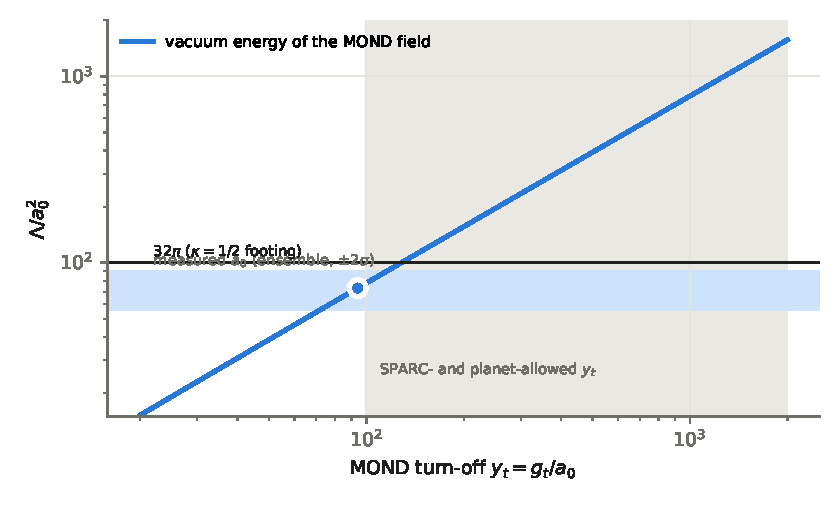
\includegraphics[width=0.78\textwidth]{fig1_paper42_band.pdf}
\caption{The MOND field's vacuum energy $\Lambda c^4/a_0^2$ against its turn-off $y_t$ (blue). Horizontal band: the value required by the observed $\Lambda$ with measured $a_0$ (dark: $1\sigma$, light: $2\sigma$); the dot marks the central solution $y_t=94$. Black line: the $\kappa=\tfrac12$ footing. Shaded: turn-offs that SPARC cannot distinguish from the exact law ($y_t\ge100$) and that the planets allow.}\label{fig:band}
\end{figure}

\section{Predictions}
\begin{enumerate}
\item \textbf{Equation of state.} If the kernel is fixed, $\rho_{\rm DE}\propto a_0^2$ at all times. A constant $a_0$ means $w=-1$ exactly. Conversely, if dark energy evolves (as DESI DR2 hints), $a_0(z)\propto\sqrt{\rho_{\rm DE}(z)}$: about $0.8\times$ today's value at $z=2.5$ on DESI's $w_0w_a$ fits. The rival reading $a_0\propto H(z)$ gives $3.7\times$. The two are separable with $\sim0.1$\,dex at $z\approx2.5$.
\item \textbf{A MOND turn-off near $10^{-8}$\,m\,s$^{-2}$, which is structurally out of reach.} Above $g_t$ the boost falls as $y^{-3}$. Near $y_t$ the boost itself is only $\nu-1\simeq1/(2y_t)\approx0.5\%$, so no galaxy-scale probe can see more than $\sim0.002$\,dex of the turn-off. For the 187 ATLAS3D early-type galaxies (JAM quality $\ge1$, $y\le38$ at $r_{1/2}$) the predicted dynamical masses move by $\sim10^{-4}$\,dex, 60 times below the sample's statistical reach and about 900 times below the 0.10\,dex stellar-population floor; SLACS lenses ($y\approx5$--20) move by $\le5\times10^{-4}$\,dex (programme lane p38). The planets show only that some turn-off exists ($y_t\le7.7\times10^5$). So $g_t$ cannot be measured independently, and Prediction~1 is the model's testable content.
\item \textbf{No zero-point $\Lambda$.} The cosmological constant is the MOND field's energy, of order $a_0^2/G$, not a quantum zero-point sum, so the $10^{122}$ problem is relocated rather than solved: any separate matter vacuum energy must still be cancelled or small.
\item \textbf{Galaxies need no dark-matter particle} (the MOND field does that work). Cosmology still needs the cold mass.
\end{enumerate}
% AUDIT: B05

\section{What is not derived}
\begin{itemize}
\item \textbf{The coefficient.} A Lean proof shows that $a_0=\tfrac12c\sqrt{G\rho_\Lambda}$ (equivalently $\Lambda A_S=32\pi^2$ with $A_S$ the area of the Schwarzschild horizon of surface gravity $a_0$) is \emph{independent} of the ingredients above. Models exist with and without it, and every coefficient $\kappa>0$ is realised. Here it is replaced by the turn-off $y_t$, a new constant.
\item \textbf{The turn-off's shape.} Steeper turn-offs ($k=3,4$) change $y_t$ for the same $\Lambda$ (167.5 and 182.4 on the $\kappa=\tfrac12$ footing).
\item \textbf{The identification itself} (dark energy = MOND vacuum energy) is a hypothesis, not a consequence of the action.
\item \textbf{The kernel's transition shape.} On SPARC the RAR kernel fits better than $\sqrt{1+1/y}$, but the preference is degenerate with the stellar mass-to-light ratio (it falls from $\Delta\chi^2=141$ to 12 as $\Upsilon_{\rm disk}$ goes from 0.5 to 0.7). This matters here: with the RAR kernel the vacuum integral converges without any turn-off, to $\Lambda c^4/a_0^2=12.99$, $5.6\times$ below the observed value (p21). The $\Lambda$ match therefore needs the quadrature kernel with a turn-off, which is the worse-fitting kernel on SPARC at fixed $\Upsilon$.
\end{itemize}
% AUDIT: B06

\paragraph{Reproducibility.} Scripts \fpath{sonnet55_push/puzzle_32pi/p21_bimond_vacuum.py}, \fpath{p25_symmetric_bimond_map.py}, \fpath{p35_kernel_tail_fix.py}, \fpath{p36_sparc_turnoff_fit.py}, \fpath{p37b_shape_vs_upsilon.py}; Lean \fpath{fable_independent_2026/lean_2026/PUZZLE_32pi_chain_2026_10_05.lean}, \fpath{PUZZLE_32pi_postulate_status_2026_10_05.lean}; figure \fpath{make_paper42_figures.py}; audit \fpath{PAPER42_audit.py}.

\small
\paragraph{References.}
[D23] Desmond, arXiv:2303.11314 (2023).
[LMS16] Lelli, McGaugh \& Schombert, AJ 152, 157 (2016).
[M99] Milgrom, Phys.\ Lett.\ A 253, 273 (1999), astro-ph/9805346.
[M09] Milgrom, Phys.\ Rev.\ D 80, 123536 (2009), arXiv:0912.0790.
[M20] Milgrom, arXiv:2001.09729 (2020).
[SJ06] Sereno \& Jetzer, MNRAS (2006).
\end{document}
